\documentclass[aps,reprint,superscriptaddress,11pt]{revtex4-2}
\usepackage{kotex}
\usepackage[HWP]{dhucs-interword}
\usepackage[dvips]{color}
\usepackage{graphicx}
\usepackage{bm}
\usepackage{amsmath}
\usepackage{tikz}
\usepackage{natbib}



\begin{document}
\title{응집물질물리실험 결과보고서 \\
\small 실험주제 : STM}

\author{HuiJae-Lee}\email{hjlee6674@inha.edu}
\affiliation{Physics Department, Inha University}

\date{\today}


\begin{abstract}
  이번 실험은 STM으로 graphite의 표면을 스캔하는 실험으로 표면을 스캔하고 FFT를 통해
  노이즈를 줄이는 과정을 통해 graphite 표면에 대해 보다 선명한 real lattice 이미지를 얻게 된다.
  실험의 결과로 graphite의 표면에 위치한 탄소 원자들이 육각형 구조로 배열을 이룬다는 사실과
  C-C 결합 길이 145 nm를 얻었다.
\end{abstract}

\maketitle

%\section[Introduction]{Introduction}
%STM의 기원은 Ricard Fyenman의 1959년 강연 "There's Plenty of Room at the Bottom: 
%An Invitation to Enter a New Field of Physics"에서 찾을 수 있다. 그는 각각의 
%원자를 뚜렷하게 보고 우리가 원하는 방식으로 배열하는 새로운 연구 분야를 
%제시했고, 그로부터 20년 후 과학자들은 STM(Scanning Tunneling Microscope)과 
%AFM(Atomic Force Microscope)의 개발로 그 목표를 달성하기 시작했다. 
%STM은 80년대 초 IBM 연구소 소속 Gerd Binning과 Heinrich Rohrer에 의해 개발되었고 
%Binning과 Rohrer는 그 공로로 86년 노벨 물리학상을 수상하였다.
%STM은 나노 스케일에서의 과학과 기술을 더욱 높은 수준으로 끌어올렸고 기초 물리학에 대한 
%이해 또한 엄청나게 발전시켰다. 그 중에서도 이번 실험에 사용할 STM은 3차원에서 표면 구조를 
%직접, 실제로 제공한다.

\section{Process}
STM을 이용한 graphite의 표면을 측정하기 위해 다음과 같은 순서로 실험을 진행하였다.
\begin{itemize}
  \item[1. ] STM에 장착되어 있던 기존의 탐침을 제거하고 STM에 전원을 인가하여 작동하는지 확인한다.
  또한 컴퓨터에서 기기를 인식하는지 확인한다.
  \item[2. ] 관찰하고자 하는 시료를 관찰에 용이한 상태로 만든다. Graphite가 존재하는 샘플을 
  꺼내고 graphite에 스카치 테이프를 붙였다 떼어 표면을 새로 만들어 낸다.
  \item[3. ] STM에 장착할 탐침을 제작한다. cutter로 탐침을 절단하고자 하는 단면에 힘을 주어
  얇게한 후 탐침을 잡아당겨 절단면의 끝부분이 날카로워지도록 한다.
  \item[4. ] 탐침과 시료를 STM에 장착한다. 탐침을 먼저 STM에 고정시킨 후 grahite이 존재하는 
  샘플을 샘플 홀더와 같이 기기에 장착한다.
  \item[5. ] 확대경을 이용해 탐침과 grahite가 닿지않는 선에서 최대한 가까워지도록 샘플의 위치를
  조절한다. 이 때 탐침과 샘플 사이 거리가 가까울 수록 후속 절차를 빠르게 진행할 수 있다.
  \item[6. ] STM을 진동 방지 상자에 넣고 컴퓨터를 통해 표면 측정을 시작한다. 
  \begin{itemize}
    \item[(1)] 컴퓨터가 STM을 인식하면 프로그램 창 상단에 있는 [Approach] 버튼을 눌러 탐침이
    시료의 표면을 측정 가능하도록 시료와 탐침 사이 거리를 조절하도록 한다. [Approach] 버튼 
    주위에 놓여져 있는 [Advance]와 [Retract] 버튼은 각각 탐침과 시료의 거리를 빠르게 좁히거나
    늘리는데 사용한다. 이 기능은 [Approach] 버튼에 비해 굉장히 빠르게 거리를 조정하므로
    눈으로 직접 보면서 사용하거나 사용을 자제해야 한다.
    \item[(2)] 표시등을 보며 탐침의 접근이 잘 진행 중인지 확인한다.
     프로그램 창 우측 하단에 세개의 표시등이 위치해 있는데 좌측부터 순서대로 적색등,
    황색등, 녹색등이다. 적색등은 탐침과 시료가 접촉하였을 때 점등된다. 황색등은 [Approach] 버튼을 
    눌러 탐침이 시료 표면에 접근 중일 때 점등되며 녹색등은 탐침이 충분히 접근하여 스캔이 가능할 때
    점등된다. 적색등이 점등된 경우, 1~6번 과정을 반복한다. 탐침과 시료에 손상이 가해졌기 때문이다.
    황색등이 점등된 경우, 탐침이 접근 중이므로 주위의 진동을 최소화하여 녹색등의 점등을 기다린다.
    \item[(3)] 위 과정들이 잘 진행되었다면 녹색등이 점등되고 컴퓨터가 자동으로 표면 스캔을 
    시작한다.
  \end{itemize}
  \item[7. ] 매끄러워 보이는 표면의 위치를 확대하여 이미지를 얻는다.
  \item[8. ] WSxM 프로그램을 이용해 얻은 이미지의 노이즈를 제거한다.
  \begin{itemize}
    \item[(1)] 이미지를 선택하고 프로그램 창 좌측 상단의 [FFT] 버튼을 눌러 Fourier 
    Transfromation을 진행한다. filter 종류를 logarithm으로 선택하여 reciprocal lattice 
    이미지를 얻는다.
    \item[(2)]  reciprocal lattice 이미지의 중앙부터 원하는 지점까지 드래그하여 
    노이즈를 줄인 real lattice 이미지를 얻는다.
  \end{itemize}
\end{itemize}

\section{Result}
STM을 통해 얻은 이미지 FIG.~\ref{fig:1}은 real lattice 이미지로 graphite의 표면을 스캔한 
결과이다. FIG.~\ref{fig:2}는 
FIG.~\ref{fig:1}을 Fourier Transfromation하여 얻은 결과이다. 이미지의 중심으로부터 주변 6곳에 
점이 찍혀있는 모습을 확인할 수 있다. 
\begin{figure}[htp]
  \centering
  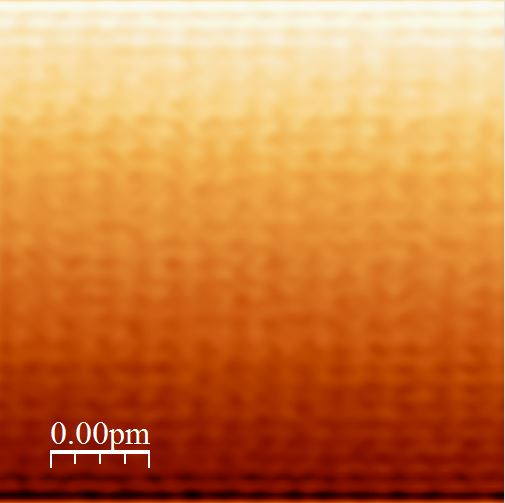
\includegraphics[scale=0.5]{fig1.jpg}
  \caption{STM으로 얻은 이미지}
  \label{fig:1}
  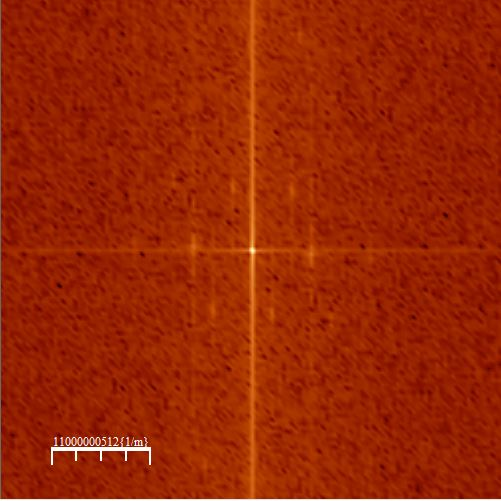
\includegraphics[scale=0.5]{fig2.jpg}
  \caption{프로그램으로 얻은 FIG.~\ref{fig:1}의 reciprocal lattice 이미지}
  \label{fig:2}
\end{figure}
FFT를 통해 얻은 reciprocal lattice 이미지로부터 노이즈가 감소한 real lattice 이미지
FIG.~\ref{fig:3}을 얻을 수 있으며 노이즈가 감소한 이미지에서는 graphite의 육각형 구조를 조금 더
선명히 볼 수 있다(FIG.~\ref{fig:4}).
\begin{figure}[htp]
  \centering
  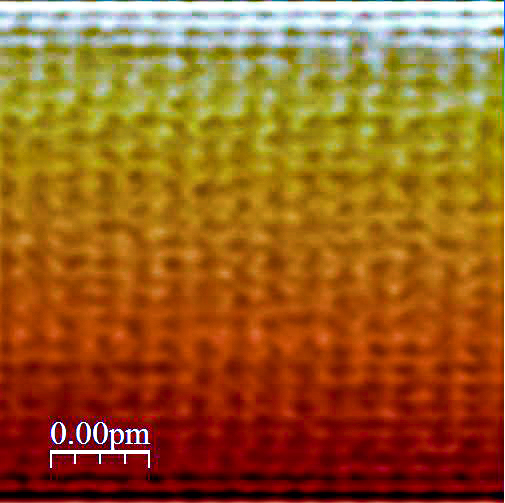
\includegraphics[scale=1]{fig3.jpg}
  \caption{노이즈가 감소한 real lattice 이미지}
  \label{fig:3}
  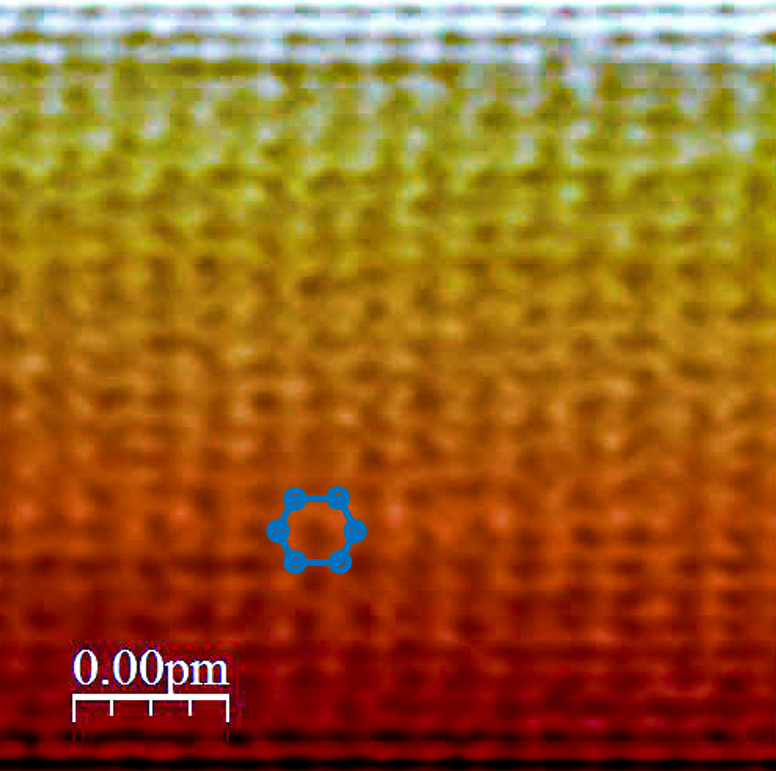
\includegraphics[scale=0.275]{fig4.png}
  \caption{real lattice 이미지에 보이는 육각형 구조}
  \label{fig:4}
\end{figure}
이 육각형 구조가 실제 graphite의 구조인지 알아보기 위해 각 꼭짓점 간의 거리를 측정하였다.
비례관계를 이용해 얻은 두 꼭짓점 간의 실제 거리는 0.145 nm이다(FIG.~\ref{fig:5}).
\begin{figure}[htp]
  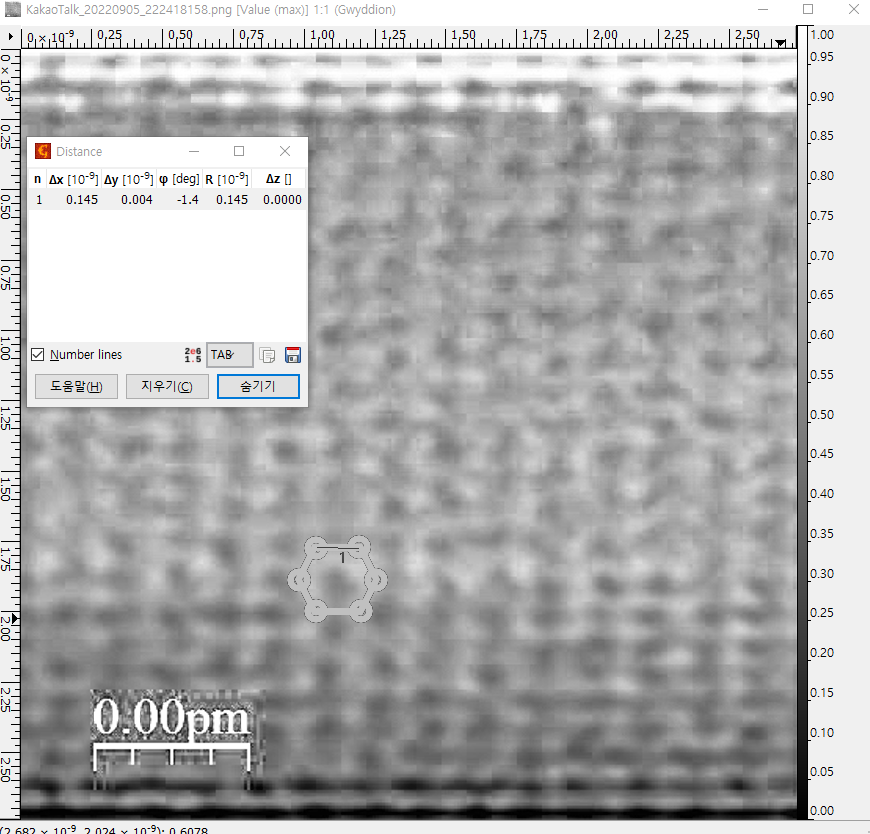
\includegraphics[scale=0.35]{fig5.png}
  \caption{육각형 구조의 꼭짓점 간 거리}
  \label{fig:5}
\end{figure}

\section{Analysis}
FIG.~\ref{fig:1}에서 보여지는 STM이 스캔한 이미지는 탐침과 표면 사이 거리가 
멀 수록 색이 진하게 표현되었다. 틈틈히 보이는 작은 검은 영역에 탄소 원자가 존재하는데
이들이 일정한 규칙성을 가지고 배열되어 있음을 짐작할 수 있다. 추가적으로 STM이 스캔하여 보여준 
이미지에 담긴 영역은 아래로 갈 수록 표면의 전체적인 높이가 감소하는 영역이었음을 유추할 수 있다.\\
Reciprocal lattice 이미지(FIG.~\ref{fig:2})는 FIG.~\ref{fig:1}의 검은 영역들이
일정한 배열을 가지고 있음을 알려준다. 노이즈를 줄이기 위해 FIG.~\ref{fig:2}에서 배열구조에 대한
최소한의 정보를 담은 영역만을 설정하여 real lattice로 표현하여 FIG.~\ref{fig:3}을 얻었다. 
FIG.~\ref{fig:3} 역시 배열구조가 선명하게 보이지는 않지만 FIG.~\ref{fig:4}와 같이 육각형 구조로
배열되어 있음을 알 수 있다. 

\begin{table}[htp]
  \centering\begin{tabular}
    {|c|c|c|c|}
    \hline
    Experimental value & Theorical value\cite{FitzerKochlingBoehmMarsh+1995+473+506} 
    & relative error \\
    \hline
    145 nm & 141.7 nm  & 2.33~\% \\
    \hline
  \end{tabular}
  \caption{C-C 결합 길이 관측 결과와 이론값의 비교}
  \label{tab:1}
\end{table}

real lattice 이미지(FIG.~\ref{fig:4})의 육각형 구조의 꼭짓점에 
탄소 원자가 위치해 있을 것이라 예상하고 탄소 원자 간의 거리를 구한 결과(FIG.~\ref{fig:5}),
실험을 통해 얻은 수치와 기존에 알려져 있던 수치가 다음과 같이 일치하는 결과를 
얻었다(TABLE.~\ref{tab:1}). \\
STM의 스캔으로 얻은 graphite의 표면 이미지가 과거 다른 조들의 이미지에 비해 
선명하지 않았고 C-C 결합거리와 기존의 이론값의 상대 오차가 2.33 \% 만큼 발생하였는데 그에 대한
원인은 진동 제어 부족이다. STM이 탐침을 시료의 표면에 가깝게 하는 과정이 상당히 오래걸려 기기 주변에서 
발생하는 진동의 영향을 적지 않게 받았을 것이다. 진동의 원인은 대부분 필자를 포함한 조원들의 
부주의성이므로 진동 방지에 대한 중요성을 더 숙지하고 조심했더라면 보다 선명한 이미지를 얻고 오차도 
더 줄일 수 있었을 것이다. 추가적으로, 탐침의 첨도를 더 높일 수 있었다면 선명한 이미지를
얻을 수 있었을 것이다. 



\section{Conclusion}
\begin{itemize}
  \item[1. ] STM으로 graphite의 표면을 측정하는 이번 실험을 통해 graphite의 탄소 원자들이
  육각형 구조로 결합한다는 사실과 graphite의 표면 탄소 원자 결합거리 141.7 nm를 직접적으로 확인하였다. 
  또한, STM을 통해 데이터를 얻고 데이터를 개선하여 실험 결과로써 도출하는 방법을 익힐 수 있었다.
  \item[2. ] 위에서 언급한 바와 같이, 진동에 대한 주의성 숙지와 탐침 제작에 대한 숙련도가 더
  쌓인 상태였다면 질적으로 더 우수한 실험 결과를 얻을 수 있었을 것이란 점에서 아쉬움이 남는다.
  \item[3. ] STM을 이용한 측정 시도는 크게 2번이었는데 첫번째 시도는 graphite의 표면을 스캔하던 중,
  탐침이 표면에 닿아 실패하였다. 두번째 시도에 이 보고서에 실린 데이터를 얻을 수 있었는데 
  탐침이 표면에 접근하는데 많은 시간이 걸려 주변 진동의 영향을 많이 받아 질이 떨어졌으리라 예상한다.
  \item[4. ] 언급한 내용들을 바탕으로, 
  \begin{itemize}
    \item[(1)] STM에 탐침과 시료를 장착할 때 탐침과 시료 사이 거리를 최소화할 수록,
    \item[(2)] 탐침의 첨도를 최대한 높일 수록,
    \item[(3)] 탐침이 표면에 접근하는 과정에서 주변의 진동을 최소화할 수록 
  \end{itemize}
  본 실험이 성공적으로 진행되었을 것이라 생각한다.
\end{itemize}

\nocite{*}
\bibliography{ref_}



%\begin{thebibliography}{9}
%\end{thebibliography}

\vfill
\end{document}